\begin{frame}{Diagram elements - Onebody Hamiltonian}
    \note{Filename: diagram\_hamiltonian01.tex}

    \renewcommand{\figurename}{Level}

    \begin{figure}
    \centering
    \parbox{0.20\textwidth}{
            \centering
            
\includegraphics[scale=0.65]{graphics/f1}
            \caption{-1}
        }
        \parbox{0.20\textwidth}{
            \centering
            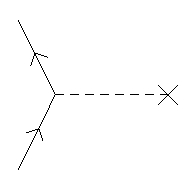
\includegraphics[scale=0.65]{graphics/f2}
            \caption{0}
        }
        \parbox{0.20\textwidth}{
            \centering
            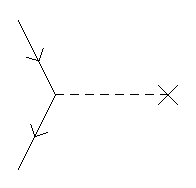
\includegraphics[scale=0.65]{graphics/f3}
            \caption{0}
        }
        \parbox{0.20\textwidth}{
            \centering
            
\includegraphics[scale=0.65]{graphics/f4}
            \caption{+1}
        }
    \end{figure}

    \begin{itemize}
        \item Horisontal dashed line segment with one vertex.
        \item Excitation level identify the number of particle/hole pairs created by the operator.
    \end{itemize}
\end{frame}

    
